
\chapter{Add labels}

\pagestyle{fancy}
\fancyhf{}
\fancyhead[OC]{\leftmark}
\fancyhead[EC]{\rightmark}
%\renewcommand{\footrulewidth}{1pt}
\cfoot{\thepage}
\label{chap:labels}

%%%%%%%%%%%%%%%%%%%%%%%%%%%%%%%%%%%%%%%%%%%%%%%%%%%%%%%%%%%
%%%%%%%%%%%%%%%%%%%%%%%%%%%%%%%%%%%%%%%%%%%%%%%%%%%%%%%%%%%

\section{Put a label next to a point}

We're going to modify our layer \textit{headquarters} by adding some labels.\\
In the \textit{Layer Styling Panel} select the layer  \textit{headquarters}.
Click the \textit{Labels} icon on the LHS of the  \textit{Layer styling Panel}.
Select “Single labels”
Label with: Head quarters
Change the settings under the various style tabs.
\begin{enumerate}[~~~1)]
	\item
	Text:
	\begin{enumerate}[~~~1)]
		\item
		Size: 7.2
		\item
		Colour: Black
	\end{enumerate}

	\item
	Buffer: 
	\begin{enumerate}[~~~1)]
		\item
		Size: 1
		\item
		Colour: White
		\item
		Opacity: 70%
	\end{enumerate}

	\item
	Placement
	\begin{enumerate}[~~~1)]
		\item
		Around point
		\item
		Distance: 1.5
	\end{enumerate}
\end{enumerate}

\begin{figure}[!h]
	\centering
	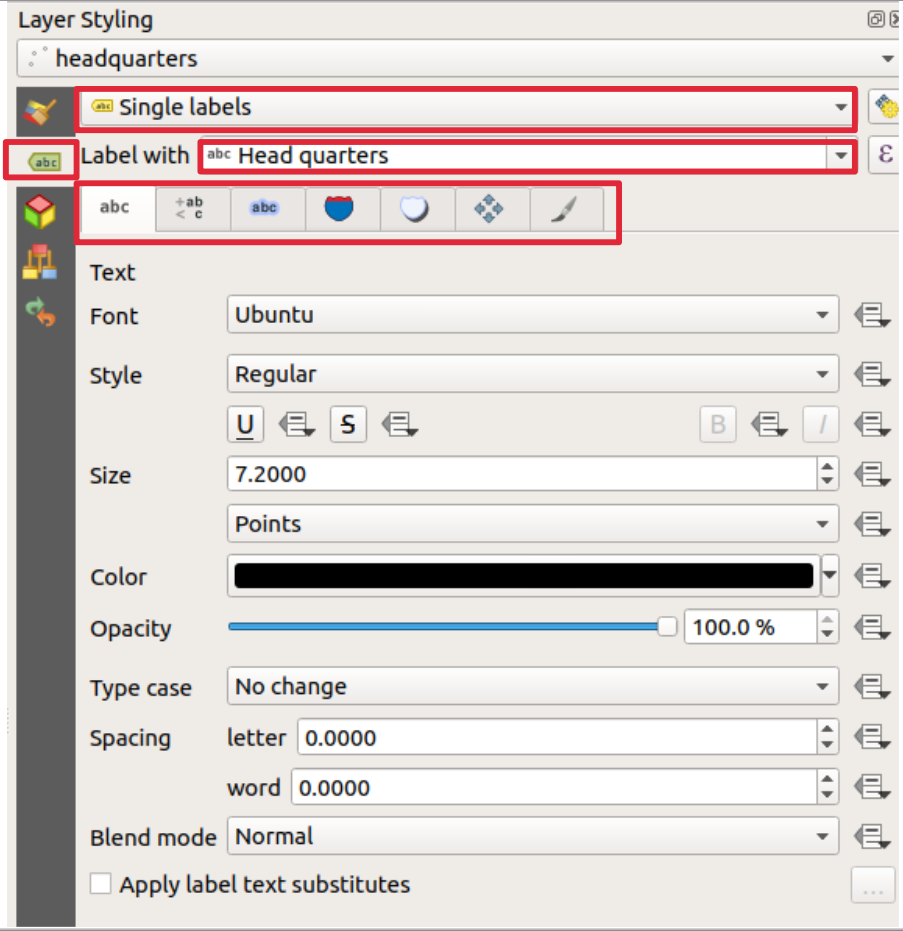
\includegraphics[width=0.4\textwidth]{images/point_label.png}
	\caption{Add label with text from field \textit{head quarters}}
	\label{ft_fig_firstfig3}
\end{figure}

\section{Using rule based labels}

Take a duplicate of the headquarters layer and rename it.\\

Let's imagine we only want to show a label for the 2 HQs that are also the Fire and Rescue HQs. We will use the boolean field $Fire\_Rescue\_HQ\_site\ in\ headquarters.csv$.\\

In the drop down click on "Single labels" and select: \textit{Rule-based labelling}. 
Can see that under "Rule" there is "(no filter)". This is where we will put our filter.  Double click on "(no filter)". 

\begin{figure}[!h]
	\centering
	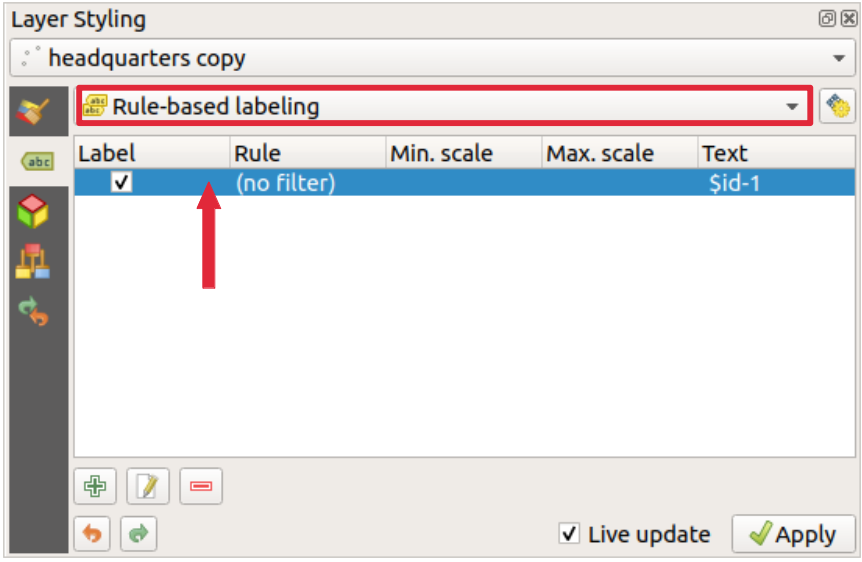
\includegraphics[width=0.35\textwidth]{images/rule_based_labels.png}
	\caption{Layer Styling panel showing Rule-based labelling}
	\label{ft_fig_firstfig3}
\end{figure}


If we know the syntax we can type the expression directly in the Filter text box. Otherwise click on the expression icon 
\begin{tabular}{@{}c@{}}
\includegraphics[width=4ex]{images/expression_icon.png}\end{tabular}
to bring up the same style form we used to select our features in the attribute table.

\begin{figure}[!h]
	\centering
	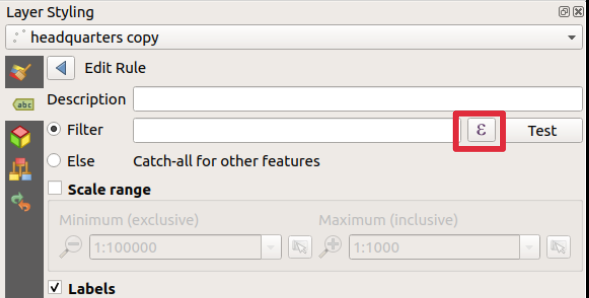
\includegraphics[width=0.4\textwidth]{images/rule_based_labels1a.png}
	\caption{Rule-based styling window. Click the expression icon to use the expression string builder form}
	\label{ft_fig_firstfig3}
\end{figure}

Use the middle pane to populate the LHS pane with the expression: \textbf{"Fire\_Rescue\_HQ\_site" ='TRUE'}. The bottom of the \textit{Expression String Builder} window will remain "Expression is invalid", until it is correct.\\

OK \& Apply \& \begin{tabular}{@{}c@{}}
\includegraphics[width=4ex]{images/blue_triangle_icon.png}\end{tabular}. Now see that only 2 labels exist on the map canvas.\\

\begin{figure}[!h]
	\centering
	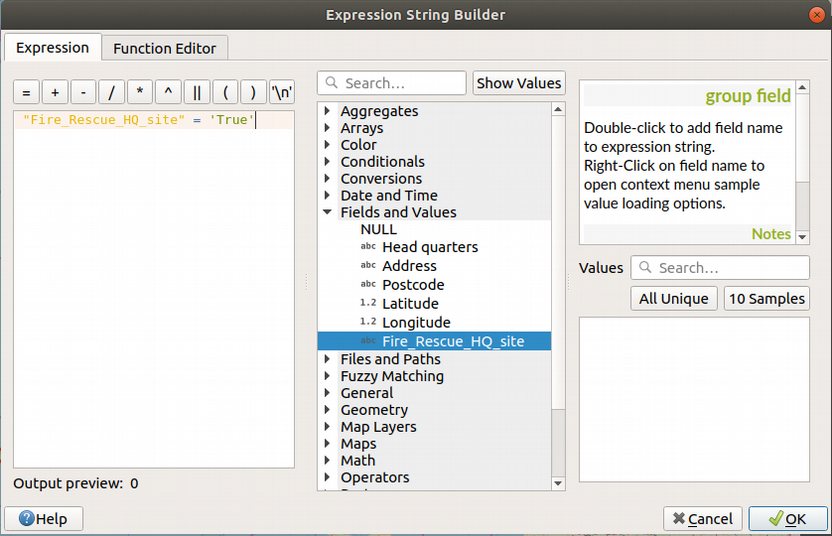
\includegraphics[width=0.5\textwidth]{images/rule_based_labels2.png}
	\caption{Expression string builder form to only have labels for locations also with Fire \& Rescue}
	\label{ft_fig_firstfig3}
\end{figure}


\section{Put a number in a point}
Take a duplicate layer of the headquarters, and rename it.\\

Going to use a unique integer from each HQ as the label, and place this at the location of the HQ. First we need to create this unique integer. I'll show you two options.

\begin{enumerate}[~~~1)]
	\item Add a new field to the layer’s attribute table

Open attribute table:
\begin{tabular}{@{}c@{}}
\includegraphics[width=4ex]{images/attribute_table_icon.png}\end{tabular} and click field calculator: 
\begin{tabular}{@{}c@{}}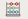
\includegraphics[width=4ex]{images/open_field_calculater_icon.png}\end{tabular}\\

In the field calculator form, you can calculate a new field using existing fields and variables of each feature. Use the search bar to find a variable that will contain a unique value, let's try "id". Great, there's a variable called \textbf{\$id}. From practice, I know \$id starts from 2 for this data, so type: \textbf{\$id - 1}.\\
Output field name: "FID"

\begin{figure}[!h]
	\centering
	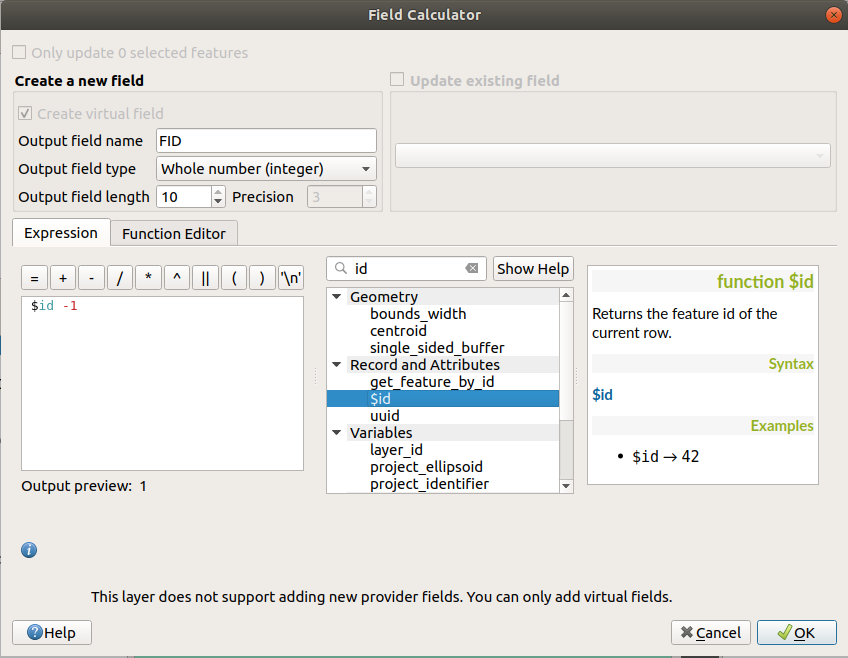
\includegraphics[width=0.48\textwidth]{images/field_calculator_form.png}
	\caption{Calculating a new field and adding to attribute table}
	\label{ft_fig_firstfig3}
\end{figure}

This new field has been added to the attribute table.\\
Close the attribute table (otherwise the new field does not seem to save)

\begin{figure}[!h]
	\centering
	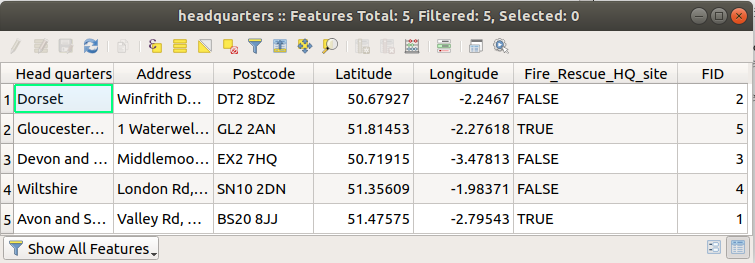
\includegraphics[width=0.55\textwidth]{images/headquarters_attribute_table.png}
	\caption{Headquaters layer attribute table with new field: FID}
	\label{ft_fig_firstfig3}
\end{figure}

{\color{gray}Additional information: To delete a field, either in the attribute table, or in \textit{Layer Properties} $\rightarrow$ \textit{Source Fields} select \textit{Toggle editting mode} \begin{tabular}{@{}c@{}}
\includegraphics[width=4ex]{images/edit_icon.png}\end{tabular}, select the field you wish to delete, then \textit{Delete field} \begin{tabular}{@{}c@{}}
\includegraphics[width=4ex]{images/delete_field_icon.png}\end{tabular}}\\

In the \textit{Layer Styling Panel}.\\
\textbf{Symbology}: No symbols\\
\textbf{Labels}: Single labels\\
\textbf{Label with}: FID\\

\null\newpage
	\item Label with expression
	
In the \textit{Layer Styling Panel}.\\
\textbf{Symbology}: No symbols\\
\textbf{Labels}: Single labels\\
\textbf{Label with}:  \begin{tabular}{@{}c@{}}
\includegraphics[width=4ex]{images/expression_icon.png}\end{tabular}\\
%\subsection{Label with expression}

In the expression dialog form, use the search bar to find a variable that will contain a unique value, let's try "id". Great, there's a variable called \textbf{\$id}. From practice, I know that \$id starts from 2 for this data, so type: \textbf{\$id - 1}.\\

\begin{figure}[!h]
	\centering
	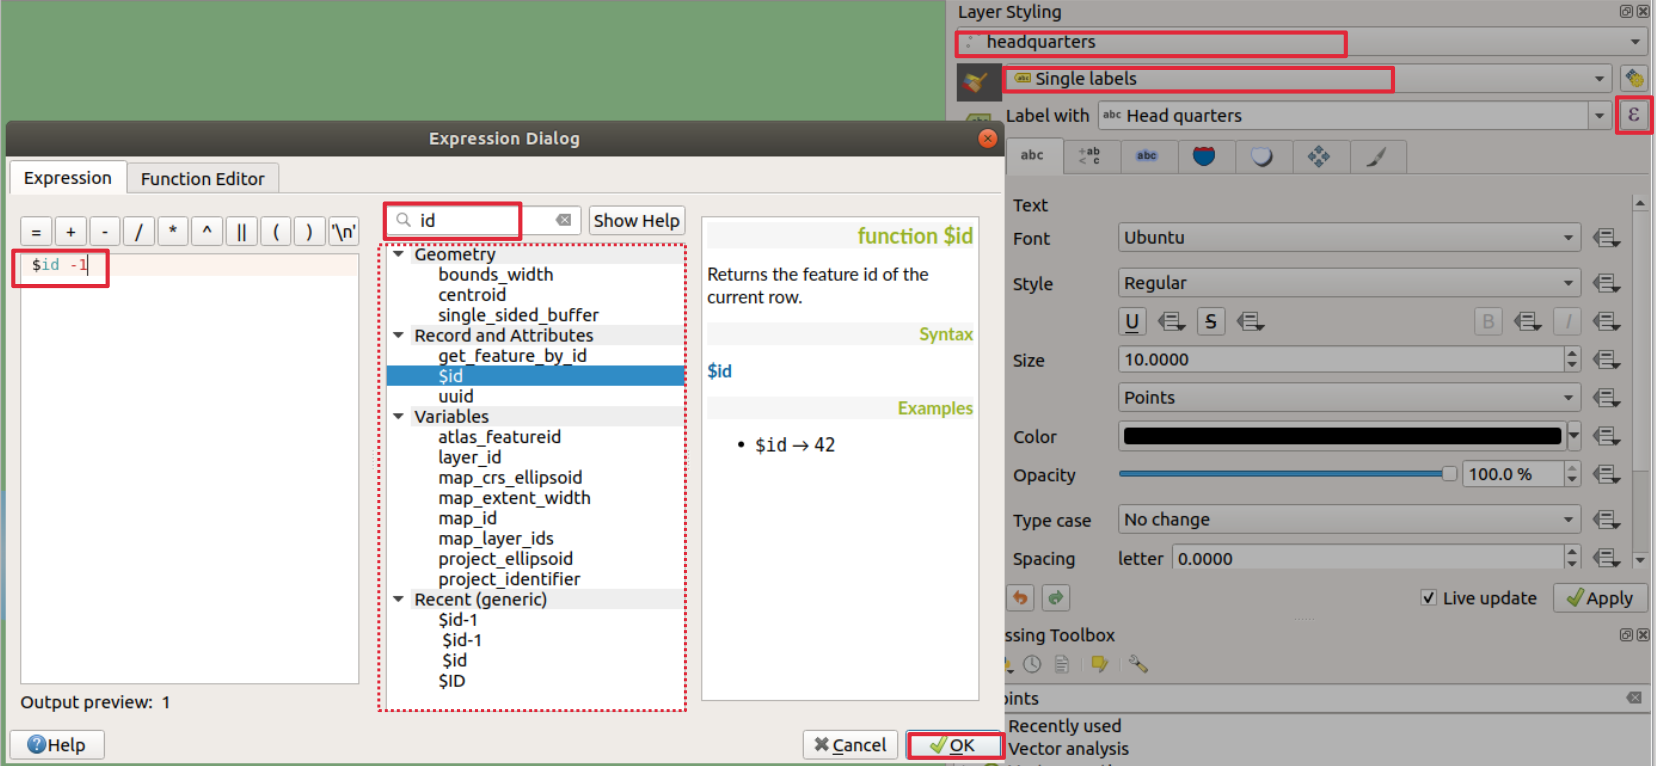
\includegraphics[width=0.74\textwidth]{images/label_with_expression.png}
	\caption{Using an expression as a label}
	\label{ft_fig_firstfig3}
\end{figure}

\end{enumerate}

You've now got your unique integer - now change the settings under the various style tabs:

\begin{enumerate}[~~~1)]
	\item
	Text:
	\begin{enumerate}[~~~1)]
		\item
		Size: 9.2
		\item
		Colour: White
		\item
		Style: Bold
	\end{enumerate}
	
	\item
	Background: 
	\begin{enumerate}[~~~1)]
		\item
		shape: Circle
		\item
		Size type: Buffer
		\item
		Fill \& boarder colour: Black
	\end{enumerate}
	
	\item
	Placement
	\begin{enumerate}[~~~1)]
		\item
		Offset from point: Central
	\end{enumerate}
\end{enumerate}

\begin{figure}[!h]
	\centering
	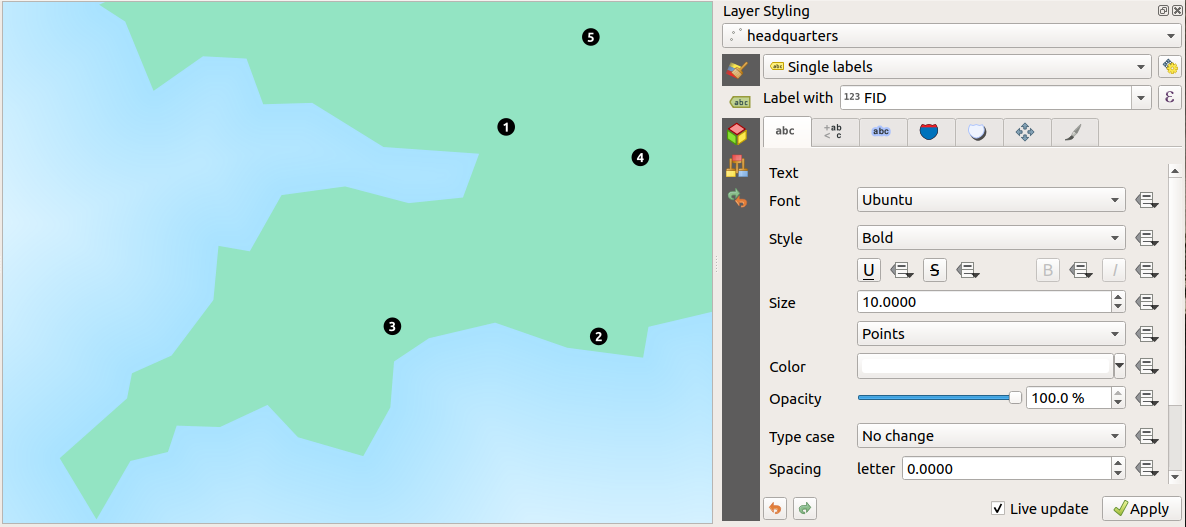
\includegraphics[width=0.47\textwidth]{images/number_in_point2.png}
	\caption{Displaying a unique number at each point}
	\label{ft_fig_firstfig3}
\end{figure}
